%%%%%%%%%%%%%%%%%%%%%%%%%%%%%
%% Styles, packages and new commands
\input{../Main/ML_Main.tex}
%%%%%%%%%%%%%%%%%%%%%%%%%%%%%
%% Edit the title page
\title{Machine Learning}
\subtitle{Module 4: Metrics}
\author[MOB]{Marc-Olivier Boldi}
\institute[HEC MSc Mgt BA]{Master in Management, Business Analytics, HEC UNIL}
\date{Spring 2025}
%%%%%%%%%%%%%%%%%%%%%%%%%%%%%
%%%%%%%%%%%%%%%%%%%%%%%%%%%%%
%%%%%%%%%%%%%%%%%%%%%%%%%%%%%
%%%%%%%%%%%%%%%%%%%%%%%%%%%%%
\begin{document}
%%%%%%%%%%%%%%%%%%%%%%%%%%%%%
\begin{frame}
  \titlepage
\end{frame}
%%%%%%%%%%%%%%%%%%%%%%%%%%%%%
\begin{frame}
\frametitle{Table of Contents}
	\tableofcontents
\end{frame}
%%%%%%%%%%%%%%%%%%%%%%%%%%%%%
%%%%%%%%%%%%%%%%%%%%%%%%%%%%%
\section{Concept}
%%%%%%%%%%%%%%%%%%%%%%%%%%%%%
%%%%%%%%%%%%%%%%%%%%%%%%%%%%%
\begin{frame}
\frametitle{Concept}
A {\bf metric} (score) is a numerical value measuring the performance of a model\\ 
\vspace{0.2cm}
To compare the different models, the metric {\it only} depends on the observed and predicted values or classes. There are metrics for regression and metrics for classification.
\begin{center}
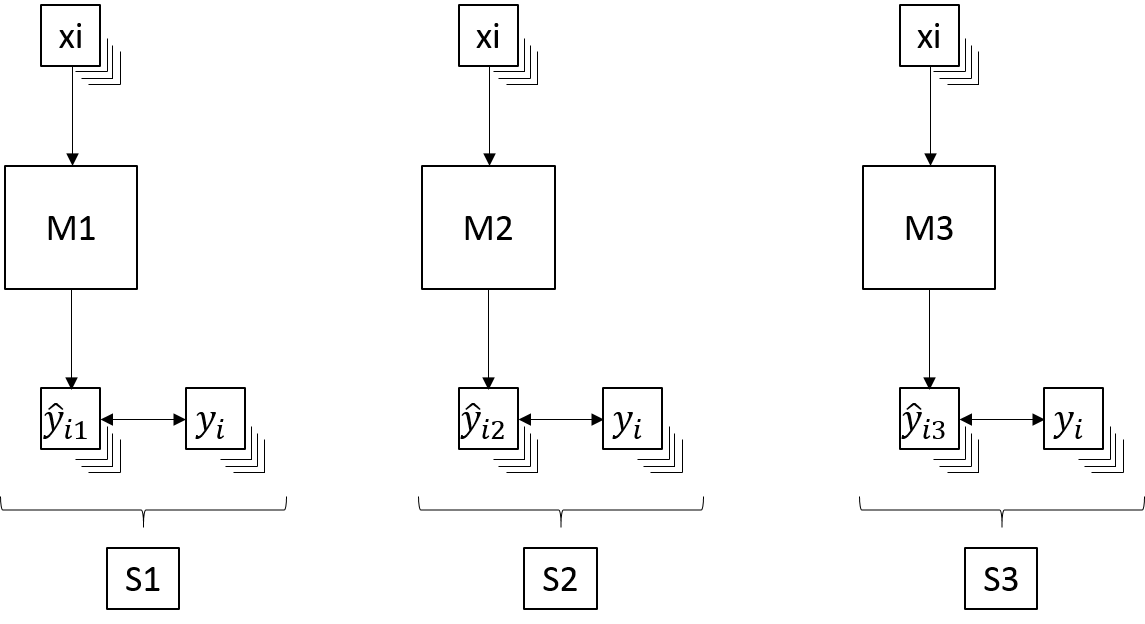
\includegraphics[width=7cm]{../Graphs/ML3.png}
\end{center}
\end{frame}
%%%%%%%%%%%%%%%%%%%%%%%%%%%%%
%%%%%%%%%%%%%%%%%%%%%%%%%%%%%
\section{Metrics for classification}
%%%%%%%%%%%%%%%%%%%%%%%%%%%%%
%%%%%%%%%%%%%%%%%%%%%%%%%%%%%
\begin{frame}
\frametitle{Metrics for classifications}
Metrics for classifications can be grouped as
\begin{itemize}
\item Metrics based on the predicted classes only (e.g., accuracy)
\item Metrics based on the predicted probabilities (e.g., AUC)
\item Metrics for binary classifications only (e.g., specificity, sensitivity, $F_1$)
\end{itemize}
\end{frame}
%%%%%%%%%%%%%%%%%%%%%%%%%%%%%
\begin{frame}[fragile]
\frametitle{Confusion matrix}
The {\bf confusion matrix} reports the frequencies of "observed" vs "predicted" classes. E.g., SVM with linear kernel and cost $C=1$, on iris data:\\
\scriptsize
\begin{verbatim}
            Reference
Prediction   setosa versicolor virginica
  setosa         50          0         0
  versicolor      0         48         2
  virginica       0          2        48
\end{verbatim}
\normalsize
All the metrics based on predicted classes can be computed from the confusion matrix. 
\end{frame}
%%%%%%%%%%%%%%%%%%%%%%%%%%%%%
\begin{frame}
\frametitle{Accuracy}
The {\bf accuracy} is the proportion of correct predictions of the model
$$
\A = \sum_i n_{ii}/\sum_{ij} n_{ij} 
$$
where $n_{ij}$ is the number in the confusion matrix at line $i$ and column $j$.\\
\vspace{0.3cm}
For the previous SVM model, the accuracy is
$$
\A = \frac{50+48+48}{50+2+48+48+2} = 0.973
$$
\end{frame}
%%%%%%%%%%%%%%%%%%%%%%%%%%%%%
\begin{frame}
\frametitle{Cohen's kappa}
{\bf Cohen's kappa} is a measure which compares the observed accuracy to the accuracy that one would expect from a random model.\\ 
\vspace{0.2cm}
The {\bf expected accuracy} from a random model is computed as the accuracy from a table containing the expected frequencies $n_{ij}$ if the model was random\footnote{The calculations are the same as for the chi-squared test for independence.}.\\ 
\vspace{0.3cm}
This expected accuracy is also called {\bf No Information Rate}.
\end{frame}
%%%%%%%%%%%%%%%%%%%%%%%%%%%%%
\begin{frame}
\frametitle{Cohen's kappa}
Suppose we have the following confusion matrix for a 3-class classification problem on $n=182$ observations:
\begin{center}
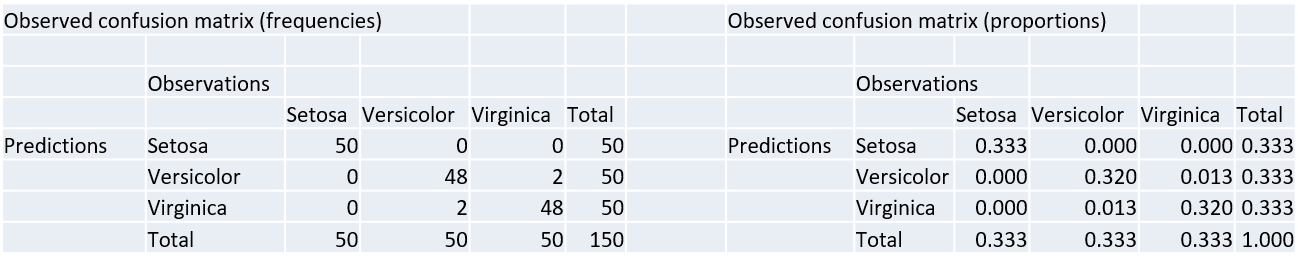
\includegraphics[width=12cm]{../Graphs/Kappa_Obs.png}
\end{center}
The {\bf observed accuracy} is 
$$
A_o = \frac{45+48+55}{182} = 0.247 + 0.264 + 0.302 = 0.813.
$$ 
\end{frame}
%%%%%%%%%%%%%%%%%%%%%%%%%%%%%
\begin{frame}
\frametitle{Cohen's kappa}
A random model would have proportions in each cell resulting from the independence between "Observation" and "Prediction". E.g.,
\begin{eqnarray*}
P(Obs=B\; \cap\; Pred=A) &=& P(Obs=B)P(Pred=A)\\
&=& 0.330 \times 0.352\\ 
&=& 0.116.
\end{eqnarray*}
Given that there are $n=182$ observations, we would expect in this cell to contain a frequency of
$$
0.166 \times 182 = 21.1.
$$
Applying this to the whole table provides the table of expected frequencies under independence.
\end{frame}
%%%%%%%%%%%%%%%%%%%%%%%%%%%%%
\begin{frame}
\frametitle{Cohen's kappa}
\begin{center}
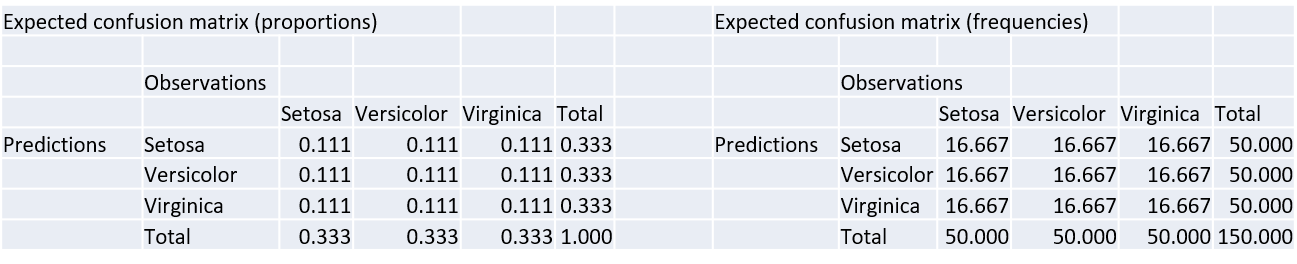
\includegraphics[width=12cm]{../Graphs/Kappa_Exp.png}
\end{center}
The expected accuracy (under independence) is 
$$
A_e = \frac{19.8+19.3+21.4}{182} = 0.109 + 0.106 + 0.117 = 0.332
$$ 
Therefore, a model without link between observations and predictions would reach an accuracy of 0.332.  
\end{frame}
%%%%%%%%%%%%%%%%%%%%%%%%%%%%%
\begin{frame}
\frametitle{Cohen's kappa}
By definition, the Cohen's kappa is
$$
\kappa = \frac{A_o - A_e}{1-A_e} 
$$
\begin{itemize}
\item $\kappa = 0$ if $A_o=A_e$ when the accuracy of the model is the same as a random model (i.e., it is not a good model).
\item $\kappa = 1$ if $A_o=1$ when the accuracy of the model is 1 (i.e., it is a good model).
\item Intermediate values are the excess of accuracy of the model over the random model, relative to the inaccuracy of the random model ($1-A_e$).
\end{itemize}
In the example,
$$
\kappa =\frac{0.813 - 0.332}{1 - 0.332} = 0.72.
$$
\end{frame}
%%%%%%%%%%%%%%%%%%%%%%%%%%%%%
\begin{frame}
\frametitle{Metrics for binary classification}
With a binary classification task (0/1):
\begin{center}
\begin{tabular}{|c|c|c||c|}
\hline
& Predict 1 & Predict 0 & Total \\
\hline
True 1 & $TP$ & $FN$ & $P$\\
\hline
True 0 & $FP$ & $TN$ & $N$ \\
\hline
\hline
Total & $PP$ & $PN$ & $M$\\
\hline
\end{tabular}
\end{center}
where\\
\scriptsize
\begin{itemize}
\item $TP$: $\#$ instances $1$ that are predicted as $1$: "true positives"
\item $FP$: $\#$ instances $0$ that are predicted as $1$: "false positives"
\item $TN$: $\#$ instances $0$ that are predicted as $0$: "true negatives"
\item $FN$: $\#$ instances $1$ that are predicted as $0$: "false negatives"
\item $P$: $\#$ instances $1$: ``positives''.
\item $N$: $\#$ instances $0$: ``negatives''.
\item $PP$: $\#$ instances predicted $1$: ``predicted positive''.
\item $PN$: $\#$ instances predicted $0$: ``predicted negative''.
\item The total number of instances is $M=TP+FP+TN+FN=P+N=PP+PN$.
\end{itemize}
\end{frame}
%%%%%%%%%%%%%%%%%%%%%%%%%%%%%
\begin{frame}[fragile]
\frametitle{Metrics for binary classification}
A logistic regression was fitted to a data set\footnote{The well known German credit data}. The positive class is ``Good''. There are 700 "Good" and 300 "Bad" in the data set.
\begin{center}
\begin{tabular}{c|c|c||c}
& Pred Good & Pred Bad & Total\\
\hline
Obs Good  & 686 & 14 & 700\\
\hline
Obs Bad   & 273 & 27 & 300\\
\hline\hline
 Total & 959 & 41 & 1000
\end{tabular}
\end{center}
Then,
$$
TP=686, \, FP=273, \, TN=27, \, FN=14\, 
$$
and
$$
P=700, \, N=300, \, PP=959, \, PN=41.
$$
\end{frame}
%%%%%%%%%%%%%%%%%%%%%%%%%%%%%
\begin{frame}
\frametitle{Sensitivity}
The {\bf sensitivity} is the proportion of correct predicted positive among the true positives:
$$
\mbox{Sens}=\frac{TP}{TP+FN}=\frac{TP}{P}
$$
It is the probability that the model recovers a positive instance:
$$
Pr\left(\mbox{model predicts positive}\;\vert\;\mbox{positive}\right).
$$
It is also referred to as {\bf recall} or {\bf true positive rate}. E.g., with the credit data
$$
Sens=\frac{686}{686+14}=0.98
$$
The model is thus very good at recovering the positive instances.
\end{frame}
%%%%%%%%%%%%%%%%%%%%%%%%%%%%%
\begin{frame}
\frametitle{Specificity}
The {\bf specificity} is the proportion of predicted negatives among the negatives:
$$
\mbox{Spec}=\frac{TN}{TN+FP}=\frac{TN}{N}
$$
Also called {\bf True Negative Rate}, it is the probability that the model recovers a negative instance:
$$
Pr\left(\mbox{model predicts negative}\;\vert\;\mbox{negative}\right).
$$
E.g., with the credit data
$$
TNR=\frac{27}{27+273}=0.09
$$
The model is poor at recovering the negative instances.
\end{frame}
%%%%%%%%%%%%%%%%%%%%%%%%%%%%%
\begin{frame}
\frametitle{Positive Predictive Value}
The {\bf precision} also called {\bf Positive Predictive Value}. It is the proportion of true positives among the predicted positive:
$$
PPV=\frac{TP}{TP+FP}=\frac{TP}{PP}
$$
The precision is the probability that the prediction is correct given that the model predicted positive:
$$
Pr\left(\mbox{positive}\;\vert\;\mbox{model predicts positive}\right).
$$
E.g., 
$$
PPV = \frac{686}{273+686} = 0.715
$$
Given that the model predicts a ``positive'', the chance it is indeed a positive is 0.715.  
\end{frame}
%%%%%%%%%%%%%%%%%%%%%%%%%%%%%
\begin{frame}
\frametitle{Negative Predictive Value}
It is the equivalent of the precision but for the negative class.
$$
NPV=\frac{TN}{FN+TN}=\frac{TN}{PN}
$$
It is the probability that the prediction is correct given that the model predicted it as negative:
$$
Pr\left(\mbox{negative}\;\vert\;\mbox{model predicts negative}\right).
$$
E.g., 
$$
NPV = \frac{27}{14+27} = 0.66
$$
Given that the model predicts a ``negative'', the chance it is indeed a negative is 0.66.
\end{frame}
%%%%%%%%%%%%%%%%%%%%%%%%%%%%%
\begin{frame}
\frametitle{Summary}
\begin{center}
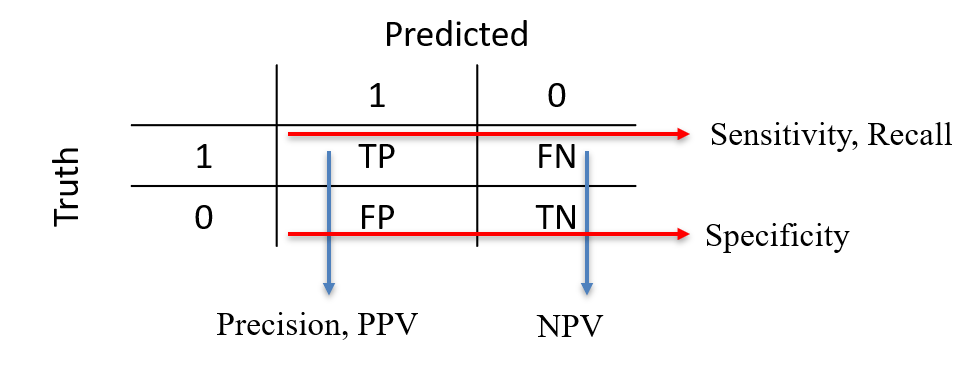
\includegraphics[width=10cm]{../Graphs/CondProb.png}\\
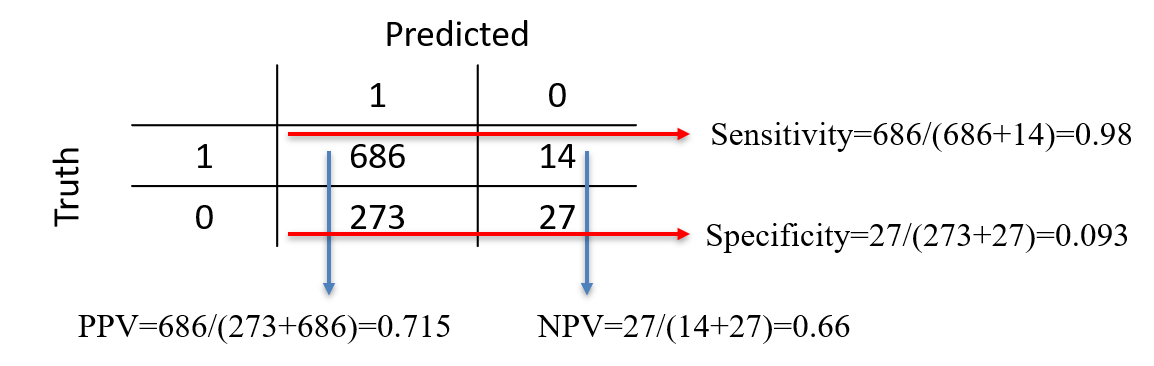
\includegraphics[width=10cm]{../Graphs/CondProb_example.png}\\
\end{center}
\end{frame}
%%%%%%%%%%%%%%%%%%%%%%%%%%%%%
\begin{frame}
\frametitle{Balanced accuracy}
One issue with the accuracy is that it is a global indicator that strongly depends on the number of positive and negative cases in the data set.\\
\vspace{0.2cm}
For example, with 700 positive instances out of 1000, a model always predicting ``Good'' would have an accuracy of 0.70: a large accuracy for such a useless model.\\
\vspace{0.2cm}
This is because of unbalance in the outcomes in the data\footnote{Note that the Cohen's kappa takes this into account.}.\\
\vspace{0.3cm} 
The {\bf balanced accuracy} is the accuracy computed {\it as if} the data were balanced. It ends up being the average between sensitivity and specificity:
$$
BA = \frac{Sens+Spec}{2}
$$
E.g., $BA=(0.98+0.09)/2=0.535$, a low value: the model cannot recover negative cases.
\end{frame}
%%%%%%%%%%%%%%%%%%%%%%%%%%%%%
\begin{frame}
\frametitle{The $F_1$ metric}
This metrics is a (harmonic) mean of the precision and the sensitivity:
$$
F_1 = 2 \times \frac{Prec\times Sens}{Prec+Sens}
$$
E.g., for the credit data $Prec = 0.715$, $Sens = 0.98$, thus
$$
F_1 = 2 \times\frac{0.715\times 0.98}{0.715+0.98} = 0.83.
$$
The limits are 
\begin{itemize}
\item $F_1 = 0$ when either Prec or Sens is 0. 
\item $F_1 = 1$ when both Prec and Sens are 1. 
\end{itemize}
The larger $F_1$, the better the model.
\end{frame}
%%%%%%%%%%%%%%%%%%%%%%%%%%%%%
%\begin{frame}
%\frametitle{The $F_1$ metric}
%The $F_1$ can be generalized to the $F_\beta$:
%$$
%F_\beta = (1+\beta^2) \frac{Prec\times Sens}{\beta^2 Prec+Sens}.
%$$
%\end{frame}
%%%%%%%%%%%%%%%%%%%%%%%%%%%%%
\begin{frame}
\frametitle{ROC curve and AUC}
The {\bf Receiver Operating Characteristic} (ROC) curve shows the sensitivities and the specificities of a model when {\it the threshold for the prediction varies}.\\
\vspace{0.3cm}
E.g., the sensitivity is 0.98, and the specificity is 0.09 with a threshold of $\lambda=0.5$: 
$$
f(x_i;\theta)=
\left\{\begin{array}{ll}
1 & \mbox{if } p(x_i;\theta) \geq \lambda,\\
0& \mbox{if } p(x_i;\theta) < \lambda .
\end{array}
\right.
$$ 
What happens when the threshold $\lambda$ ranges from 0 to 1?
\begin{itemize}
\item If $\lambda=0$, no cases are predicted as $0$, thus $Sens=1$ and $Spec=0$.
\item If $\lambda=1$, no cases are predicted as $1$, thus $Sens=0$ and $Spec=1$.
\end{itemize}
\end{frame}
%%%%%%%%%%%%%%%%%%%%%%%%%%%%%
\begin{frame}
\frametitle{ROC curve and AUC}
The ROC curve is obtained when $\lambda$ varies between 0 and 1, $Spec=x$, and $y=Sens$. The specificy (x-axis) is usually in the reverse order.
\begin{center}
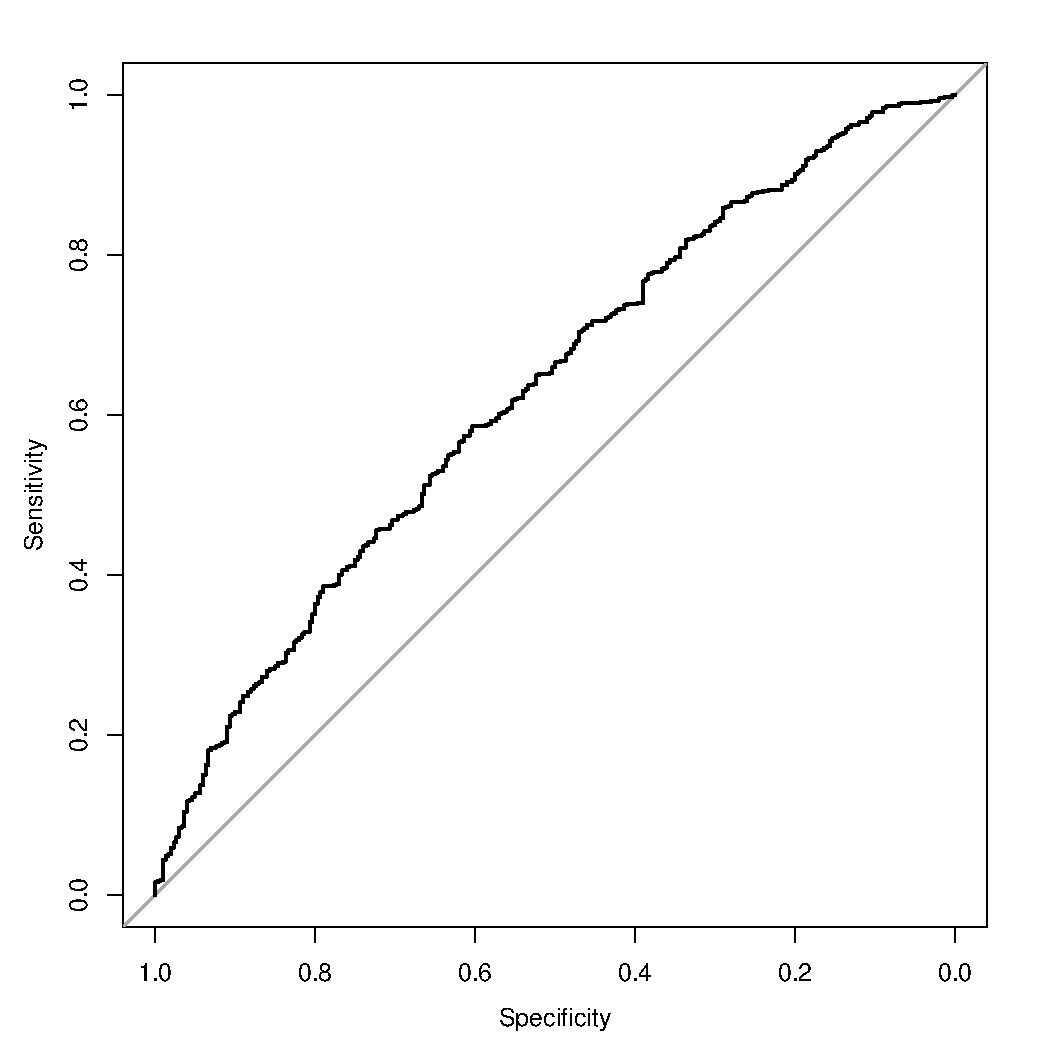
\includegraphics[width=6cm]{../Graphs/ROC_curve.pdf}
\end{center}
\end{frame}
%%%%%%%%%%%%%%%%%%%%%%%%%%%%%
\begin{frame}
\frametitle{ROC curve and AUC}
A perfect model has large sensitivity {\bf and} specificity {\bf for all} $\lambda$ (except $0$ and $1$). This corresponds to a single point in the upper left corner of the ROC.\\
\vspace{0.2cm}
The diagonal in gray corresponds to the random model. The further the curve up that diagonal, the better the model. \\
\vspace{0.2cm}
The {\bf Area Under the Curve} (AUC) is the area between the diagonal and the ROC curve. The larger it is, the better the model is.\\
\vspace{0.2cm}
E.g., $AUC=0.628$.\\
\vspace{0.2cm}
The ROC curve provides a way to {\bf tune} the threshold for the prediction under unbalanced class: select the threshold with maximum balanced accuracy (Youden Index point). See later.
\end{frame}
%%%%%%%%%%%%%%%%%%%%%%%%%%%%%
%%%%%%%%%%%%%%%%%%%%%%%%%%%%%
\section{Metrics for regression}
%%%%%%%%%%%%%%%%%%%%%%%%%%%%%
\begin{frame}
\frametitle{Root Mean Squared Error (RMSE)}
The {\bf RMSE} is the square root of the mean of the squares of the errors of prediction:
$$
RMSE = \sqrt{\frac{1}{n} \sum_{i=1}^n \left\{y_i - f(x_i;\theta)\right\}^2},
$$
The lower the RMSE, the better the model.
\end{frame}
%%%%%%%%%%%%%%%%%%%%%%%%%%%%%
\begin{frame}
\frametitle{MSE and MAE}
Other metrics:
\begin{itemize}
\item The {\bf Mean Squared Error} (MSE) is the RMSE without the square root
$$
MSE = RMSE^2
$$
It is obviously equivalent to the RMSE.
\item The {\bf Mean Absolute Error} (MAE) is the average of the absolute errors:
$$
MAE = \frac{1}{n}\sum_{i=1}^n|y_i -f(x_i;\theta)|
$$
\end{itemize}
\end{frame}
%%%%%%%%%%%%%%%%%%%%%%%%%%%%%
\begin{frame}
\frametitle{RMSE and MAE}
Like the median to the mean, the MAE is more robust than the RMSE:
\begin{itemize}
\item One large error only will make the RMSE large.
\item The MAE is less influenced by one error.
\end{itemize}
In practice, with:
\begin{itemize}
\item Model 1: mostly small errors except a few large ones,
\item Model 2: only average errors, no large one.
\end{itemize}
Then, we will probably have
\begin{eqnarray*}
MAE(M1) &<& MAE(M2)\\
RMSE(M2) &<& RMSE(M1)
\end{eqnarray*}
\end{frame}
%%%%%%%%%%%%%%%%%%%%%%%%%%%%%
\begin{frame}[fragile]
\frametitle{The $R^2$}
In the ML context, the $R^2$ ({\bf $R$ squared}) is the square of the correlation between the observations and the predictions. 
$$
R^2 = cor^2(y,f(x;\theta))
$$
The $R^2$ is bounded between 0 and 1. The larger the $R^2$, the better the model.\\
\vspace{0.3cm}
The $R^2$ is an attempt to approximate / replace the usual $R^2$ of a linear regression. However, these two must not be confounded because they will often be different (though conveying the same idea).
\end{frame}
%%%%%%%%%%%%%%%%%%%%%%%%%%%%%
%%%%%%%%%%%%%%%%%%%%%%%%%%%%%
\section{Final words}
%%%%%%%%%%%%%%%%%%%%%%%%%%%%%
%%%%%%%%%%%%%%%%%%%%%%%%%%%%%
\begin{frame}
\frametitle{Final words}
\begin{itemize}
\item There exist plethora of metrics with advantages and drawbacks. 
\item Some can be interpreted (accuracy, sensitivity, etc.), others cannot and are used only to compare models ($F_1$, $RMSE$, etc.).
\item It is important to have a {\bf baseline model} to compare the metric (e.g., random model for classification, average for regression).
\item For regression, a {\bf scatterplot of the observations $y_i$ versus the predictions $f(x_i;\theta)$} allows to analyze in more details the model quality. It is a must do!
\end{itemize}
\end{frame}
%%%%%%%%%%%%%%%%%%%%%%%%%%%%%
\end{document}




%%%%%%%%%%%%%%%%%%%%%%%%%%%%%
%%%%%%%%%%%%%%%%%%%%%%%%%%%%%
%%%%%%%%%%%%%%%%%%%%%%%%%%%%%
%%%%%%%%%%%%%%%%%%%%%%%%%%%%%
%%%%%%%%%%%%%%%%%%%%%%%%%%%%%
%%%%%%%%%%%%%%%%%%%%%%%%%%%%%
%%%%%%%%%%%%%%%%%%%%%%%%%%%%%
%%%%%%%%%%%%%%%%%%%%%%%%%%%%%
%%%%%%%%%%%%%%%%%%%%%%%%%%%%%
%%%%%%%%%%%%%%%%%%%%%%%%%%%%%
%%%%%%%%%%%%%%%%%%%%%%%%%%%%%
\begin{frame}
\frametitle{Classifications metrics based on the predicted probabilities}
All the previous metrics are based on the confusion matrix: observed and predicted classes.\\ 
\vspace{0.3cm}
Other metrics are based on the predicted probabilities. These bring a more detailed information on the model, like about its robustness or stability. Two equally good models in terms of predicted classes (e.g., same accuracy), may be very different in terms of predicted probabilities (one may be more stable or bring more certainty than the other).
\end{frame}
%%%%%%%%%%%%%%%%%%%%%%%%%%%%%
\begin{frame}
\frametitle{Entropy}
The {\bf entropy} is a general measure which compares the prediction of a model and the true instance. Like before, let $0/1$ be the negative/positive classes. Assume also that the model returns a probability given the features $x_i$ of instance $i$, 
$$
0 \leq P(Y_i=1|x_i) \leq 1,
$$
that we write $p_i$ for short. Let $y_i$ be the true class of instance $i$. Then the entropy is defined as
$$
E = -\sum_{i=1}^n y_i \log(p_i) + (1-y_i)\log(1-p_i).
$$
\end{frame}
%%%%%%%%%%%%%%%%%%%%%%%%%%%%%
\begin{frame}
\frametitle{Entropy}
Because either $y_i$ or $1-y_i$ is zero, the contribution of $i$ to the cross-entropy is
$$
\left\{
\begin{array}{ll}
-\log(p_i), & \mbox{if } y_i=1,\\
-\log(1-p_i) & \mbox{if } y_i=0.
\end{array}
\right.
$$ 
Thus, if the model is good at predicting $i$, it will assign a large $p_i$ if $y_i=1$, and a small $p_i$ (i.e. a large $1-p_i$) if $y_i=0$. Therefore, if the model is good at predicting $i$, its contribution to the entropy will be negatively large.\\
\vspace{0.2cm}
The {\it smaller} the entropy, the {\it better} the model.
\end{frame}
%%%%%%%%%%%%%%%%%%%%%%%%%%%%%
\begin{frame}
\frametitle{Entropy}
E.g., with the credit data, for instance 1, we have $p_1=0.84$ and $y_1=1$ (good), thus its contribution to the entropy is 
$$
-\log(0.84) = 0.179.
$$ 
If the model would have predicted with $p_1=0.51$ (still making a correct prediction but with much less certainty), then its contribution would have been
$$
-\log(0.51) = 0.673.
$$ 
This is much larger, and the model would then be judged less good.\\
\vspace{0.2cm}
In addition:
\begin{itemize}
\item Average instead of sum can be used (different sample size)
\item $\log_2$ instead of $\log$ can be used.
\end{itemize}
\end{frame}
%%%%%%%%%%%%%%%%%%%%%%%%%%%%%
\begin{frame}
\frametitle{Entropy for multiclass problem}
The entropy can be used for multiclass classifications. Let $p_i^c$ be the probability assigned to class $c$ by the model for instance $i$, then the entropy is
$$
E=-\sum_{i=1}^n \sum_{c=1}^C q(y_i,c) \log(p_i^c)
$$
where
$$
q(y, c) = \left\{
\begin{array}{ll}
1, & \mbox{if } y=c,\\
0, & \mbox{otherwise}.
\end{array}
\right.
$$
\end{frame}
%%%%%%%%%%%%%%%%%%%%%%%%%%%%%
\begin{frame}[fragile]
\frametitle{RMSE}
{\bf Example}: with the Facebook data, the outcome {\tt log(Lifetime.Post.Consumers)} is predicted with all the other variables using a linear regression. The RMSE is $0.709$:\\
\tiny
\begin{verbatim}
> fb.lm <- lm(log(Lifetime.Post.Consumers)~Page.total.likes + Type + Category + Post.Month + Post.Weekday + Post.Hour + Paid, 
+                 data=fb.dat.tr)
> pred.lm <- predict(fb.lm, newdata=fb.dat.te)
> (rmse.lm <- sqrt(mean((pred.lm - log(fb.dat.te$Lifetime.Post.Consumers))^2)))
[1] 0.7089739                                                                     $
\end{verbatim}
\normalsize
The RMSE is not meant to be interpreted in itself. It is a metric which allows to compare models. Below, the RMSE for the (unpruned) tree on the same sets:\\
\tiny
\begin{verbatim}
> fb.rt <- rpart(log(Lifetime.Post.Consumers)~Page.total.likes + Type + Category + Post.Month + Post.Weekday + Post.Hour + Paid, 
+                data=fb.dat.tr)
> pred.rt <- predict(fb.rt, newdata=fb.dat.te)
> (rmse.rt <- sqrt(mean((pred.rt - log(fb.dat.te$Lifetime.Post.Consumers))^2)))
[1] 0.7669044                                                                                                            $
\end{verbatim}
\normalsize
The linear regression did better than the regression tree for these data.
\end{frame}
%%%%%%%%%%%%%%%%%%%%%%%%%%%%%
\begin{frame}[fragile]
\frametitle{MSE and MAE}
To illustrate the difference between RMSE and MAE, we use the {\tt cdata2} set\footnote{Source: Statistical Methods for Social Sciences, Third Edition by Alan Agresti and Barbara Finlay (Prentice Hall, 1997); with modifications} containing 
\begin{itemize}
\item outcome: {\tt crime}, violent crimes per 100,000 people in 51 US states (in year ??)
\item feature 1: {\tt poverty}, percent of population living under poverty line, 
\item feature 2: {\tt single}, percent of population that are single parents.
\end{itemize}
Three models are compared:\\
\scriptsize 
\begin{verbatim}
mod <- lm(crime ~ poverty + single, data=cdata2)
mod2 <- lm(crime ~ poly(poverty,2) + poly(single,2), data=cdata2)
mod.rp <- rpart(crime~poverty+single, data=cdata2)
\end{verbatim}
\normalsize
\end{frame}
%%%%%%%%%%%%%%%%%%%%%%%%%%%%%
\begin{frame}
\frametitle{MSE and MAE}
The 3 graphs below show the absolute values of the errors made by the models:
\scriptsize
\begin{center}
\includegraphics[width=10cm]{../Graphs/crime_resid.pdf}
\begin{tabular}{l | ccc}
& LM & LM with quad & RT \\
\hline
RMSE & 371 & 336* & 351 \\
RMSE (without State 51) & 270 & 280 & 211*\\
MAE & 203 & 177 & 137*\\
\hline
\end{tabular}
\end{center}
*Best model
\normalsize
\end{frame}
%%%%%%%%%%%%%%%%%%%%%%%%%%%%%
\begin{frame}[fragile]
\frametitle{The $R^2$}
In the ML context, the $R^2$ ({\bf $R$ squared}) is the square of the correlation between the observations and the predictions. 
$$
R^2 = cor(y,f(x;\theta))
$$
The $R^2$ is bounded between 0 and 1. The larger the $R^2$, the better the model.\\
\vspace{0.3cm}
The $R^2$ is an attempt to approximate / replace the usual $R^2$ of a linear regression. However, these two should not be confounded because they will often be different (though conveying the same idea).\\
\vspace{0.3cm}
The linear model and the tree model on the facebook data:
\scriptsize
\begin{verbatim}
> cor(pred.lm, log(fb.dat.te$Lifetime.Post.Consumers))^2
[1] 0.3814113
> cor(pred.rt, log(fb.dat.te$Lifetime.Post.Consumers))^2
[1] 0.2809646
\end{verbatim}
\normalsize
\end{frame}
%%%%%%%%%%%%%%%%%%%%%%%%%%%%%
